\documentclass{article}
\usepackage[utf8]{inputenc}
% Language setting
% Replace `english' with e.g. `spanish' to change the document language
\usepackage[english]{babel}

% Set page size and margins
% Replace `letterpaper' with `a4paper' for UK/EU standard size
\usepackage[a4paper,top=2cm,bottom=2cm,left=3cm,right=3cm,marginparwidth=1.75cm]{geometry}

% Useful packages
\usepackage{amsmath}
\usepackage{graphicx}
\usepackage{subfig}
\usepackage{comment}
\usepackage[colorlinks=true, allcolors=blue]{hyperref}
\usepackage{placeins}
\usepackage{listings}
\usepackage[super]{nth}
\lstset{frame=tb,
  language=c++,
  aboveskip=5mm,
  belowskip=5mm,
  showstringspaces=false,
  columns=flexible,
  basicstyle={\small\ttfamily},
  numbers=none,
  numberstyle=\tiny\color{blue},
  keywordstyle=\color{red},
  commentstyle=\color{green},
  stringstyle=\color{orange},
  breaklines=true,
  breakatwhitespace=true,
  tabsize=3}

\title{Assignment 3: Refactoring the Design\\
of an Existing Project\\
\large Software Design and Modelling}

\author{Daniele Gasparini, Mattia Monari, Sergiu Gheorghita}
\date{\nth{25} November 2022}

\begin{document}

\maketitle

\section{Project Selection}
For the project selection each of us proposed some University projects we made in the previous semester whose design required a refactor. We ended up selecting Mattia's project called "Sorting Algorithms Visualized Through Images"(SAVTI), because it will be used as starting point of his BSc thesis(he is an Erasmus student) and a deep refactoring is needed to make his life easier since as it is today the project presents some design anti-pattern that must be removed.

\section{Project Description}
\textcolor{red}{Qua Tia ci mettiamo uno screen del progetto e descrivi cosa fa, poi metti il link al video youtube.}
\section{Refactoring Goals}
The refactoring we made had two main goals. The first one is to remove code smells inside the code, for this purpose we used SonarQube to detect part of the code whose design could be imporved. 
(\textcolor{red}{addActionListeners in MainWindow and AdvancedSettings})\\
The second one is to make the code more readable since the project presents complexity flaws in some classes which have very long methods.

\section{Refactoring examples}

\subsection{Fixing naming flaws}
By looking at the SonarQube report, the first thing we refactor was the naming of local variables, in this case we used a capital letter to represent a local variable so we decide to use a more readable variable for the RGB indexes instead.

\begin{comment}
\begin{figure}[!htb]
   \begin{minipage}{0.5\textwidth}
     \centering
     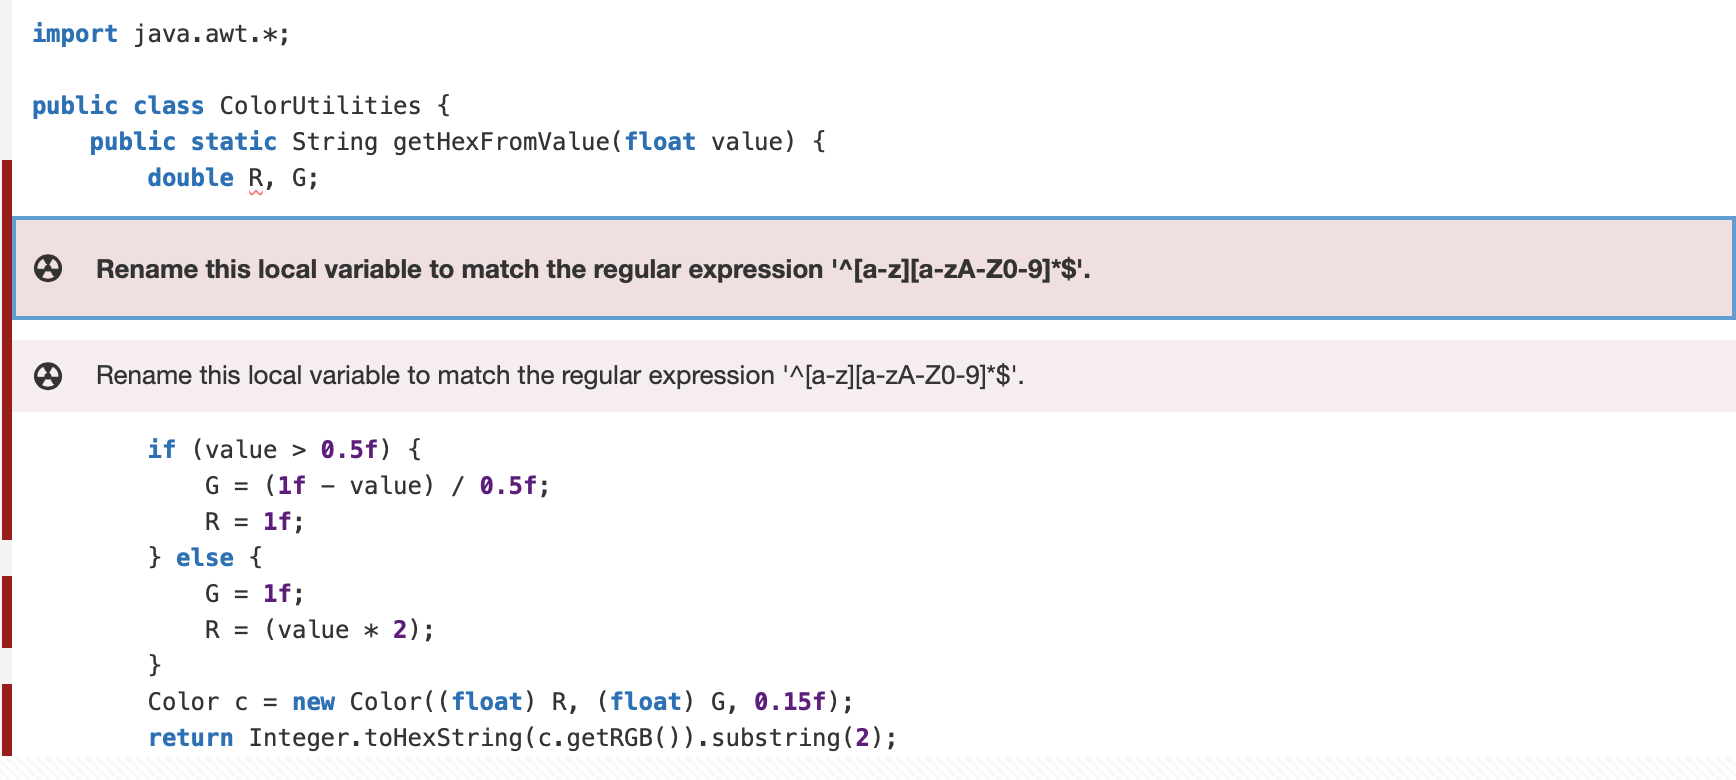
\includegraphics[width=1\linewidth]{Rename/Rename1.png}
   \end{minipage}\hfill
   \begin{minipage}{0.5\textwidth}
     \centering
     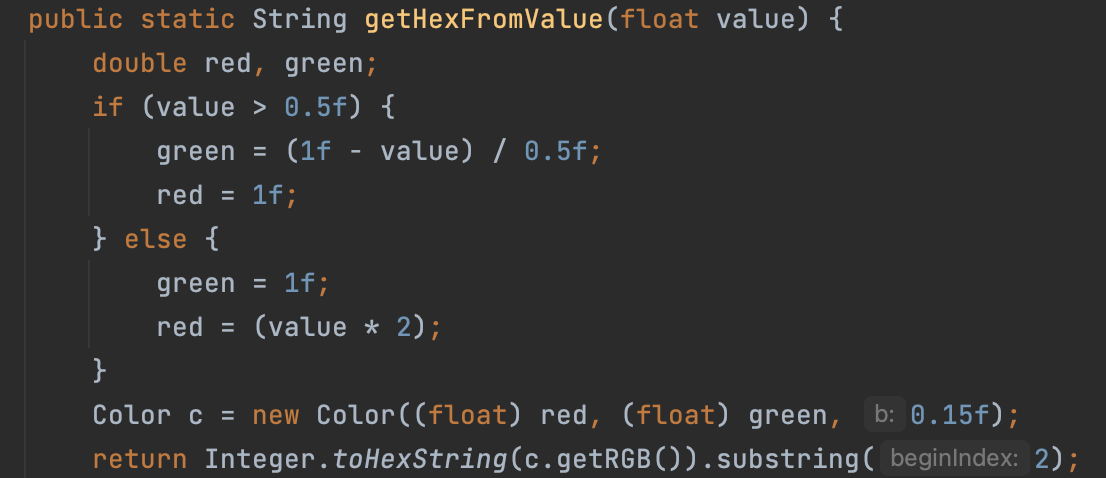
\includegraphics[width=1\linewidth]{Rename/Rename2.png}
   \end{minipage}
   \caption{Rename Local Variable and Method Parameters}\label{fig:Rename}
\end{figure}
\end{comment}
\begin{lstlisting}[caption={Fixing naming flaws},captionpos=b]
public static String getHexFromValue(float value) {
        double red, green; // before they were r and g
        if (value > 0.5f) {
            green = (1f - value) / 0.5f;
            red = 1f;
        } else {
            green = 1f;
            red = (value * 2);
        }
        Color c = new Color((float) red, (float) green, 0.15f);
        return Integer.toHexString(c.getRGB()).substring(2);
    }
\end{lstlisting}
\subsection{Collapsable If statement should be merged}
To solve this issue we merged the collapsable if statement to increase readability, for this reason we first merged the two condition as one by using the logical AND(&&).\\
Then, since the same sentence was used inside numerous classes(UserSettings, AdvancedSettings and MainWindow) we decided to reduce the coupling of the class and create a method called isOutputDirectory, inside the class UserSettings, whose purpose is to check that the output directory is not null and check that effectively it is a directory.
\begin{lstlisting}[caption={Old Implementation},captionpos=b]
if (userSettings.getOutputDirectory() != null){
    if (userSettings.getOutputDirectory().isDirectory()){
\end{lstlisting}


\begin{lstlisting}[caption={New Implementation},captionpos=b]
public boolean isOutputDirectory() {
        return getOutputDirectory() != null && getOutputDirectory().isDirectory();
    }
    
\end{lstlisting}

\begin{lstlisting}[caption={Application of the new implementation},captionpos=b]
if (userSettings.isOutputDirectory())
            try {
                Desktop.getDesktop().open(userSettings.getOutputDirectory());
            } catch (IOException e) {
                ErrorUtilities.SWW();
            }
\end{lstlisting}

\begin{comment}

\begin{figure}[!htb]
     \centering
     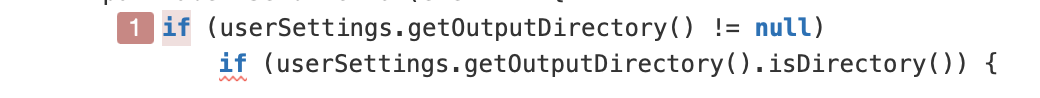
\includegraphics[width=1\linewidth]{CollapsableIF/CollapsableIF1.png}
     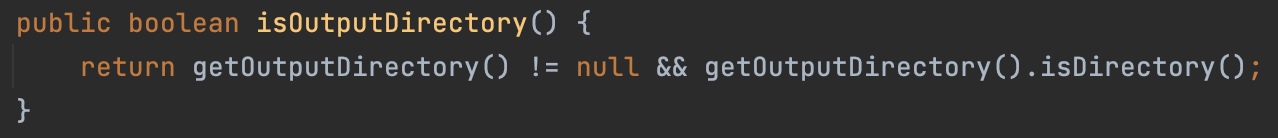
\includegraphics[width=1\linewidth]{CollapsableIF/CollapsableIF2.png}
     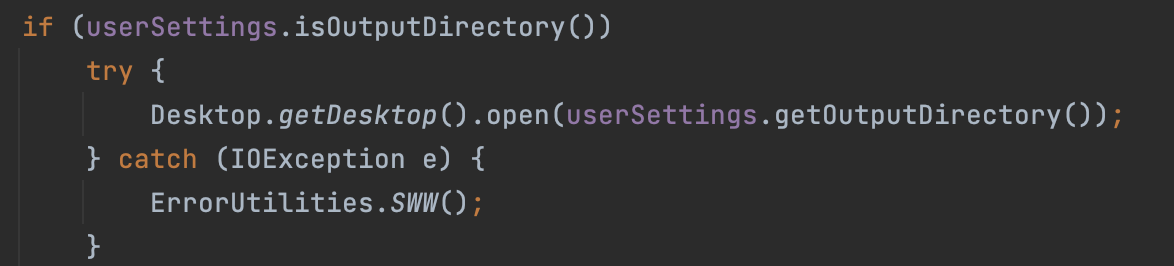
\includegraphics[width=1\linewidth]{CollapsableIF/CollapsableIF3.png}
     \caption{Collapsable If statement}
\end{figure}
\end{comment}

\subsection{Private fields only used as local variables in methods should become local variables}

In this case the private field is initiated with a builder, for this reason the tool thinks it is only used inside a method, but in reality it is initiated in the constructor by the method initComponents, this is already a form of refactoring, because instead of having a huge amount of parameters to initialize a method is used for it.

\subsection{Documentation}
To increase readability and comprehension of the project we added java docs in that parts of the program whose structure was more complex and for all the classes we created to improve the design.\\
As an example we put below the documentation we implements for the LoadSongCommand, to do it we followed JavaDocs rules.

\begin{lstlisting}[caption={Adding JavaDocs},captionpos=b]
/**
 * LoadSongCommand is used to create the command to load songs.
 *
 * @author Daniele Gasparini && Mattia Monari && Sergiu Gheorghita
 * @version 2022.11.17
 */
public class LoadSongCommand implements Command{
    MainWindow mainWindow;
    UserSettings userSettings ;
    /**
     * Constructor for LoadSongCommand class.
     * @param userSettings are the settings that will be changed after the load of the song
     */
    public LoadSongCommand(UserSettings userSettings, MainWindow mainWindow) {
        this.userSettings = userSettings;
        this.mainWindow = mainWindow;
    }
}
\end{lstlisting}
\begin{comment}
\begin{figure}[!htb]
    \centering
    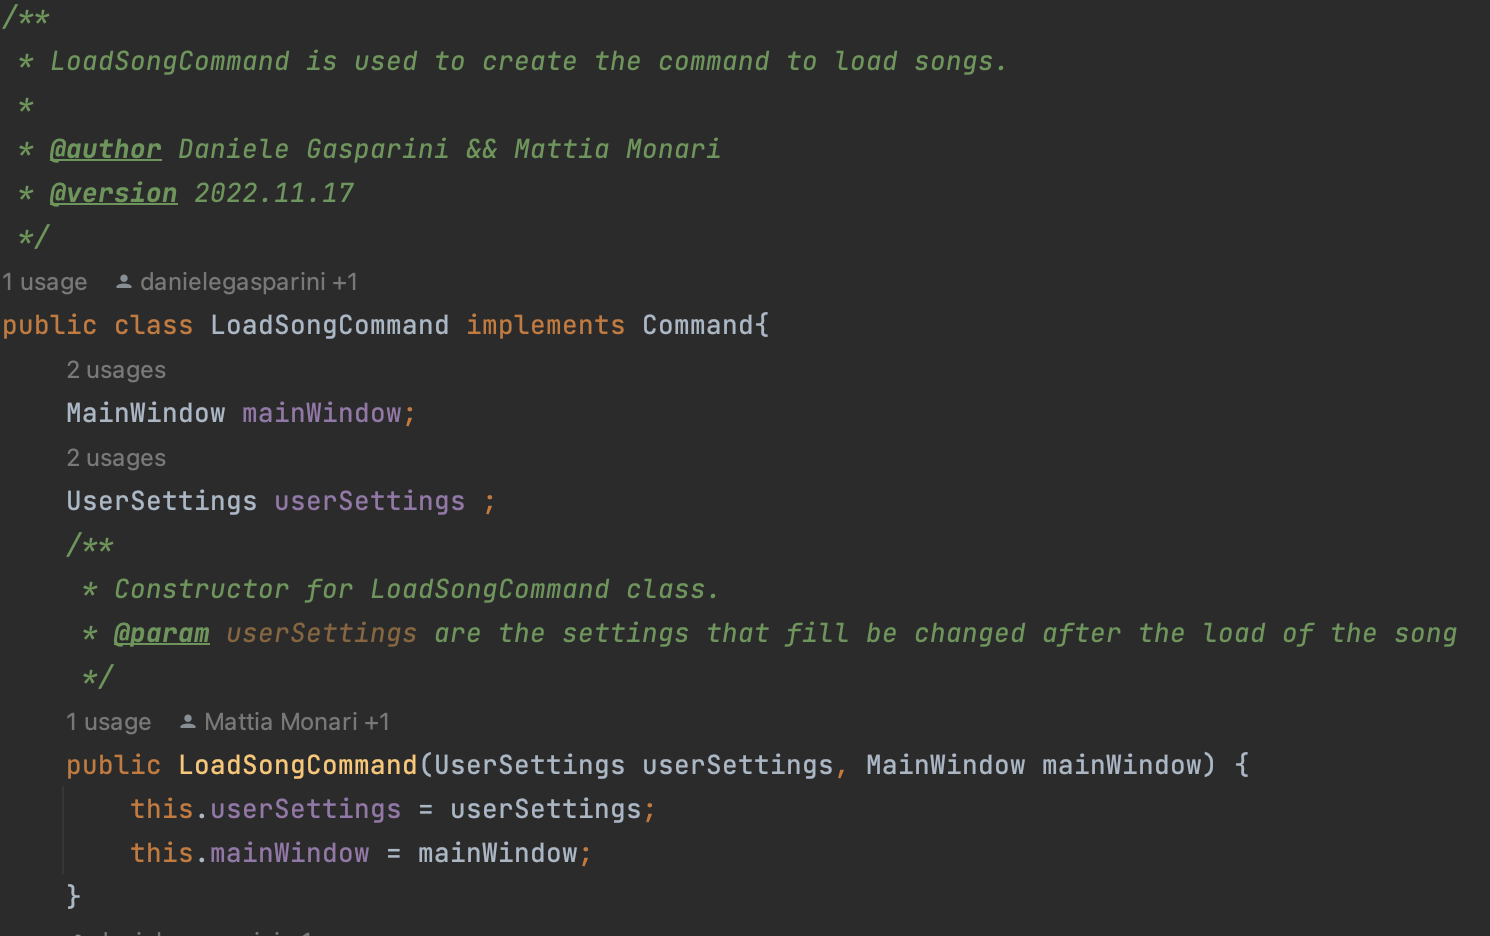
\includegraphics[width=1\linewidth]{Documentation/Documentation1.png}
    \caption{Caption}
    \label{fig:my_label}
\end{figure}

\end{comment}






\subsection{God classes and complexity flaws}
The majority of our work was to reduce the complexity of some God classes, which had a very high coupling and that presents some very long methods whose Cognitive complexity exceded the limit of 15 imposed by SonarQube.
We are talking about classes MainWindow and AdvancedSettings.\\
Our goal was to reach strong intra-class cohesion and loose inter-class coupling. 
For this reason in the case of MainWindow, whose purpose is to manage the GUI of the project, we made three distinct works.\\
First, we reduced the coupling of the class by creating two subclasses called MainVBox and MainMenu, one is responsible for the management of the main page buttons while the second one is responsible for the management of the drop down menu.\\
Then, we modified the method addEventListener, whose  purpose was to add a listener for each of the button inside the GUI. This method had a cognitive complexity of 55 and was composed by 257 lines of code, in pills it added a new event listener for each button by using lambda expression as shown in the snippet below.\\

\begin{lstlisting}
private void addEventListeners() {
        cleanButton.setOnAction(e -> {
            image.clearImage();
            imageView.setImage(null);
             deleteAllPreviousFiles(userSettings);
         });
\end{lstlisting}
The first modify we applied was to create a method for each EventListenr, so to reduce the complexity of the addEventListener method.

\begin{lstlisting}
private void cleanImageListener() {
         cleanButton.setOnAction(e -> {
             image.clearImage();
             imageView.setImage(null);
             deleteAllPreviousFiles(userSettings);
         });
     }
     
private void addEventListeners() {
         cleanImageListener();
         setAdvancedSettingsListener();
         loadImageListener();
         loadSongListener();
         setOutputPathListener();
         setDarkModeListener();
         randomShuffleListener();
         sortImageListener();
         burstModeToolTipListener();
         setBurstModeListener();
         clickToPathListener();
    }
\end{lstlisting}
Solved this smell we had to reduce the coupling of the class, for this reason we applied the Command pattern and the principle of separation of concerns, which usually results in breaking an app into layers.
For doing this we followed this scheme.

\begin{figure}[!htb]
    \centering
    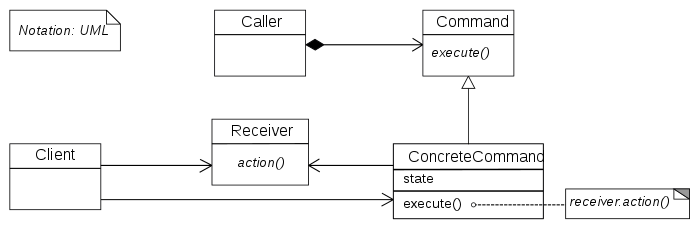
\includegraphics[width=1\linewidth]{700px-Command_pattern.svg.png}
    \caption{Command Pattern}
    \label{fig:my_label}
\end{figure}
\newpage
We build an interface Command that was implemented by each concrete command, which represents a command to execute when a button is pressed.
Each concrete command then have a receiver the CommandAction, that is used by the Client to perform the command.
Here is a snippet of the code implementation.
\begin{lstlisting}[caption={Command},captionpos=b]
public CleanImageCommand(TiledImage image, UserSettings userSettings, javafx.scene.image.ImageView imageView) {
        this.image = image;
        this.userSettings = userSettings;
        this.imageView = imageView;
    }
    @Override
    public void execute() {
        image.clearImage();
        imageView.setImage(null);
    }
\end{lstlisting}

\begin{lstlisting}[caption={Reciever},captionpos=b]
public class CommandAction extends AbstractAction {
    private final Command command ;
    public CommandAction(final Command command) {
        super();
        this.command = command;
        }
    @Override
    public void actionPerformed(ActionEvent e) {command.execute();}
}
\end{lstlisting}

\begin{lstlisting}[caption={Client},captionpos =b]
 private void addEventListeners() {
    mainVBox.getCleanButton().setOnAction(
                                e -> new CleanImageCommand(
                                    image, userSettings, imageView)
                                    .execute());
\end{lstlisting}
In this way we have also increased the cohesion, since we developed a set of classes responsible to execute the command of each button and we reduced the amount of work made by the god class MainWindow.\\
\textcolor{red}{Qua metterei il numero di righe della classe prima e dopo e la complessità del metodo addEventListener dopo il refactoring}

We used the same approach to improve the readability and the reduce the complexity of the class AdvancedSettings.
\textcolor{red}{Qua Tia metterei cosa hai fatto ieri}\\

\textcolor{red}{Non mi ricordo, avevi afatto altro te? Forse riguardo Classes that override "clone" should be "Cloneable" and call "super.clone()}\\
\textcolor{red}{Poi si può aggiungere la parte dei test}\\
\section{Refactoring testing} 
Come abbiamo testato che il codice funzionasse ancora?
\section{Difficulties}
Dire che nel caso dei primi 4 punti non abbiamo trovato molte difficoltà nell'implementazione poichè abbiamo solo dovuto modificare delle variabili, mentre nel caso della god class abbiamo dovuto fare più un lavoro di porgettazione per cercare di capire come modificare il codice senza andare a comprometterne la corretta esecuzione.

\section{Conclusion}
Add Testing
Add Enum for Literal Duplication in method choice, when we have to select between the different sorting algorithms.
Improve documentation.
Se hai altre idee aggiungi.
\end{document}
